\section{Obtaining an Unbiased Upsilon Sample}

Another way of looking at the $\Upsilon(1S)$ is through the
$\Upsilon(2S) \to \pi^+\pi^- \Upsilon(1S)$ cascade.  The recoil mass
of the two pions has a resolution of 1.5 MeV, so combinatoric
backgrounds can be highly suppressed and the sideband is nearly
linear.  But most importantly, the two pions can be chosen to satisfy
both the trigger and the database event filter, so that the
distribution of $\Upsilon(1S)$ events from the cascades study is
completely unbiased.  All decays of the $\Upsilon(1S)$ will have equal
efficiency, even completely invisible decays to two neutrinos.

One might ask if a similar study can be done for the other resonances:
unfortunately, they cannot.  The $\Upsilon(3S)$ is inaccessible
because the $\Upsilon(4S)$ has a very large decay width to $B\bar{B}$,
which overwhelms any di-pion cascades, and the $\Upsilon(3S) \to
\pi^+\pi^- \Upsilon(2S)$ produces pions with momenta $\le$ 90 MeV, for
which the tracking efficiency is poor.  Also, it isn't worthwhile
adding $\Upsilon(3S) \to \pi^+\pi^- \Upsilon(1S)$ to the
$\Upsilon(1S)$-cascade sample, as this mode adds only 12\% more
events.

There are two differences between $\Upsilon(1S)$ events from the
cascade sample and $\Upsilon(1S)$ events from the database dataset or
unfiltered dataset.  The first is a slight boost due to the recoil of
the two pions, but the maximum $\beta$ and $\gamma$ for the
$\Upsilon(1S)$ is 0.058 and 1.0033, respectively.  Another is the
possibility of track confusion with the pions.  An $\Upsilon(1S)$
track might overlap one of the pion tracks and go undiscovered, or two
tracks could be fitted to one pion, where one of them is identified as
the pion and the other is assumed to belong to the $\Upsilon(1S)$.
Both of these effects would be captured in a Monte Carlo simulation,
so $\Upsilon(2S) \to \pi^+\pi^- \Upsilon(1S)$ Monte Carlo is passed
through the same analysis as data.  Measurements from cascade Monte
Carlo can be compared with measurements from direct $\Upsilon(1S)$
Monte Carlo, and this can be used to determine a translation factor.

After two tracks in the event have been identified as belonging to the
cascade pions, they are excluded from the calculation of all cut
variables, \dxy, \dz, \pone, and \visen, and I directly measure the
cut efficiency by asking how many $\Upsilon(1S)$ events pass and how
many fail.  Ideally, I would exclude pions from the trigger as well,
but the low-level trigger variables are not available in the database
dataset.  Instead, I will bound the trigger efficiency by measuring a
looser cut and a tighter cut.

\subsection{Constraints on the Two Pion Tracks}

As a reminder, the following is a set of sufficient conditions for an
event to appear in the database dataset (see page
\pageref{wonderfuldiscovery}):
\begin{enumerate}
  \item the event passes a hardware trigger,
  \item it has two or more quality tracks,
  \item it has \hotvisen\ $>$ 4\% \ecom, and
  \item it passes \lfourdec.
\end{enumerate}
I need to choose pion tracks such that the above criteria are
satisfied by the pions alone, leaving the $\Upsilon(1S)$ free to decay
however it likes.

The first criterion can be satisfied by requesting only events which
pass the TwoTrack trigger, and then making sure that my pions alone
generate the two AXIAL tracks needed to satisfy that trigger line.  An
independent study of trigger tracking efficiency [\ref{cite:inga}]
found that if a track is reconstructed in software and has a
transverse momentum ($p_T$) $>$ 150 MeV, an AXIAL track is found at
the same $\phi$ ($\pm$ 5$^\circ$) with 99.93 $\pm$ 0.07\% efficiency.
Therefore, I will require all of my pions to have $p_T$ $>$ 150 MeV.

I am also interested in $\Upsilon(1S)$ events that pass some trigger
requirements.  After the pions guarantee two AXIAL tracks, the Hadron
trigger line only requires 1 additional AXIAL track and 1 CBLO.  All
the trigger lines that I am interested in require at least 1 AXIAL
track and 1 CBLO from the $\Upsilon$, so I acquire another sample of
di-pion cascades that passes the Hadron trigger, with the same
restrictions on pion tracks.  This way, some of my measurements can
evade the TwoTrack prescale.

I will call these two cascades samples ``little'' (from the TwoTrack
trigger line) and ``big'' (from the Hadron trigger line).  The little
sample is completely unbiased, and the big sample is biased in a way
that partly simulates the trigger.

Criteria \#2 and \#3 can be satisfied by requiring the two pions to be
quality tracks.  The energy of all quality tracks (assuming each to
have the mass of a charged pion) is included in \visen, and the
kinematics of the decay gives the two recoil pions 563 MeV.  The 4\%
threshold is 401 MeV, so this is always automatically satisfied.

A sufficient condition for \lfourdec\ is to require two tracks with
the following cuts (on quantities saved after pattern recognition but
before track fitting).  I require the two pion tracks to satisfy them.
\begin{itemize}
  \item The track must have some Z information (meaning that it
    reached the stereo layers of the DR, which is equivalent to the
    $p_t$ cut),

  \item it must have more than 40\% of its expected number of hits,

  \item $|\cos\theta|$ $<$ 0.93,

  \item $\chi^2$ $<$ 20 $\times$ the number of degrees of freedom, and

  \item it must approach the DR origin within 2.5 cm in XY and 15 cm
    in Z.
\end{itemize}

\subsection{Excluding Cascade Pion Curlers}

There is one last consideration to make before measuring cut
efficiencies: while the tracks identified as pions have been excluded
from the calculation of all $\Upsilon(1S)$ variables, a pion might
complete a full orbit around its gyration circumference and yet remain
in the detector to be measured again.  Such circular loops are
identified by the track recognition software as two (or more) tracks,
known as ``curlers.''  Because of the vertexing requirements I placed
on the pions, I always identify the track associated with the first
half-orbit.

Curlers can be eliminated from the cascades sample by cutting on the
pions' $p_z$.  The arclength (in XY projection) of an orbit is given
by
\begin{equation}
  2\pi \, \frac{p_T}{3\times 10^{-4} \, \cdot \, 1.4 \mbox{T}} \,
  \frac{\mbox{T cm}}{\mbox{MeV}}
\end{equation}
and the speed of the particle (in XY projection, $c=1$) by
\begin{equation}
  \frac{p_T}{\sqrt{{m_\pi}^2 + |\vec{p}|^2}}
\end{equation}
so the time to complete a half-orbit is
\begin{equation}
  \frac{2\pi}{4.2} \, \sqrt{{m_\pi}^2 + |\vec{p}|^2} \,
  \frac{\mbox{cm}}{\mbox{MeV}}\mbox{ (in units of cm).}
\end{equation}
Similarly, the time for the particle to move a distance $L$ in the Z
direction is
\begin{equation}
  \frac{\sqrt{{m_\pi}^2 + |\vec{p}|^2}}{p_z} \, L
\end{equation}
so the particle completes a half-orbit as it translates a distance $L$
in the Z direction if its momentum Z-component is
\begin{equation}
  \frac{2.1}{\pi} \, L \, \frac{\mbox{MeV}}{\mbox{cm}} \mbox{.}
\end{equation}
The axial section of the DR is 90 cm long in Z: this corresponds to a
$|p_z|$ of 60 MeV.  I will only accept cascade pions with a $p_z$
outside of this range.

\subsection{Recoil Mass Peak and Sideband Subtraction}

Now that I have chosen pairs of tracks which guarantee inclusion in my
sample, I use the following algorithm to reconstruct a recoil mass
peak:
\begin{enumerate}
  \item Calculate
    \begin{equation}
      m_{\pi\pi \mbox{\scriptsize -rec}} = \sqrt{(2
        E_\subs{beam} - \sqrt{|\vec{p}_1|^2 + {m_\pi}^2} -
	  \sqrt{|\vec{p}_2|^2 + {m_\pi}^2})^2 - |\vec{p}_1 +
	      \vec{p}_2|^2}
    \end{equation}
  for each pair of good tracks with momenta $\vec{p}_1$ and
  $\vec{p}_2$ at their intersection point in XY.  Each pair of tracks
  must also have opposite charges.

  \item From the set of all $m_{\pi\pi \mbox{\scriptsize -rec}}$
  combinations that are within 20 MeV of the $\Upsilon(1S)$ mass,
  intersect each other within 5 mm of the beamspot in XY and 5 cm in
  average Z (with a 2.5 cm tolerance for missing each other in Z),
  I randomly choose one.  If the set is empty, I skip the event.
\end{enumerate}

The random choice is introduced in step \#2 to make sure that the
combinatoric background doesn't peak under the signal.  Figure
\ref{cascades_recoilmass} is a plot of the recoil mass, showing the
9.454--9.472 GeV signal region and the 9.441--9.480 GeV sideband.
(The sideband includes events from both sides of the peak, excluding
the signal region.)

\begin{figure}[p]
  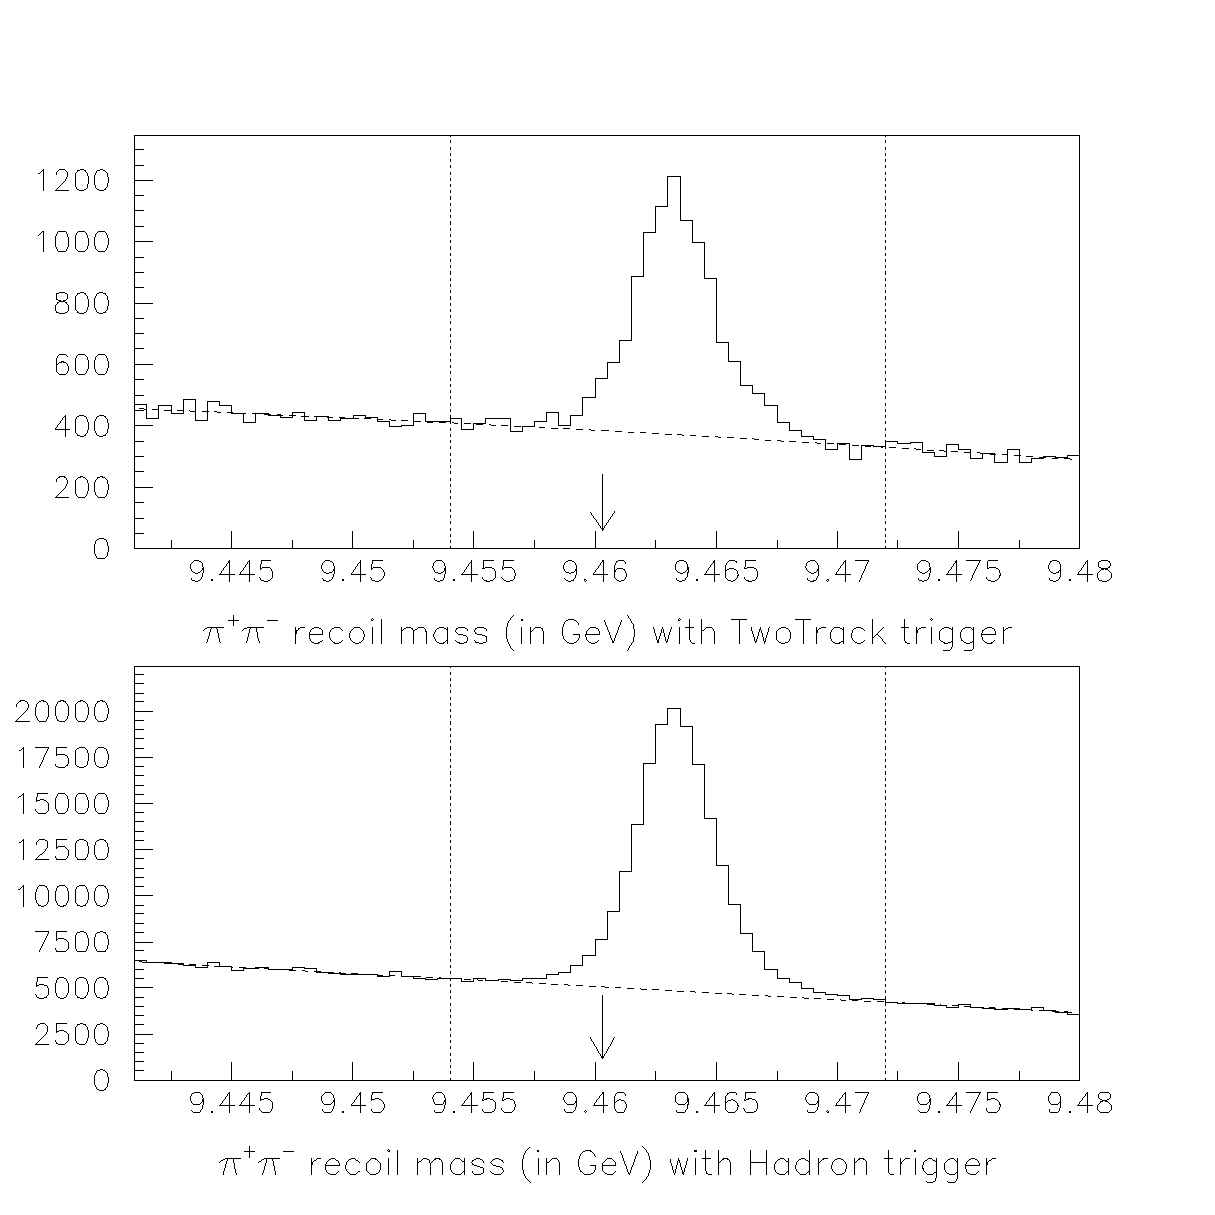
\includegraphics[width=\linewidth]{plots/cascades_recoilmass}
  \caption{\label{cascades_recoilmass} Recoil mass of the two pions in
  $\Upsilon(2S) \to \pi^+\pi^- \Upsilon(1S)$, from the TwoTrack
  trigger line (top) and from the Hadron trigger line (bottom).
  Dotted lines separate signal from sideband, and the dashed lines are
  quadratic fits to the sideband.  The arrows point to the true mass
  of the $\Upsilon(1S)$.}
\end{figure}

The combinatoric background in Figure \ref{cascades_recoilmass} is a
smooth distribution whose characteristic width is much greater than
the 39 MeV-wide plot window.  It can therefore be expanded as a
polynomial.  The distribution looks linear, but I want to bound the
error I incur from truncating the polynomial.  To do this, I use the
following fit function:
\begin{multline}
  f(m; c_0, c_1, c_2) = c_0(1) + c_1 (m - 9.458357142857055) + \\
  + c_2 (m^2-18.92233477371051 m+89.51347812358851) \label{cascades:eqn_fitfunc}
\end{multline}
where $m$ is the di-pion recoil mass, $c_0$, $c_1$, and $c_2$ are the
fit parameters.  (Yes, all of those digits are necessary!)  The three
parenthesized polynomials were chosen to be orthogonal to each other
in the sideband region, so that the fit parameters are uncorrelated
and can be individually varied for a systematic error.

I use the best-fit of the sideband to Equation
\ref{cascades:eqn_fitfunc} to interpolate under the peak, and
integrate for the number of events in the sideband and the number of
combinatoric background events in the signal region.  The ratio of
these tells me how to subtract sideband from signal, which I do to
produce plots of every variable that defines the hadron event type.
Cut efficiencies are read off the plots, and errors in $c_0$, $c_1$,
and $c_2$ are propagated into those efficiencies.  In every fit, the
quadratic term is consistent with being zero, as the background
distribution is nearly linear.  This uncertainty in $c_2$ is the
truncation error I wanted to determine.

\section{Minimal and Maximal Triggers}

With an unbiased sample of $\Upsilon(1S)$ events, I can find the
efficiency of any cut independently of all the others.  That is,
except for the trigger: the number of AXIAL tracks is not available in
the database dataset, so I cannot subtract two and recalculate the
trigger decision.  Unfortunately, I do need to know the trigger
efficiency independently of all other cuts, and I need to know the
efficiency of all other cuts with the trigger applied.  Therefore, I
must construct something like the trigger out of information which is
available to me.  (Here, the trigger in question is ``Hadron or RadTau
or ElTrack.'')

I construct two such things: what I call the ``minimal trigger,'' which
is a necessary condition for the trigger to pass an event, and the
``maximal trigger,'' which is a sufficient condition.  The efficiency
of the minimal trigger will be greater than the efficiency of the true
trigger, and the efficiency of the maximal trigger will be less than
the efficiency of the true trigger.  (The true trigger efficiency is
close to 100\%, so I will only really need the maximal trigger for
trigger efficiency measurements.  But for measurements with the
trigger applied, I will need both.)

After the two pions generate two AXIAL tracks, the Hadron trigger line
additionally requires 1 AXIAL track and 1 CBLO from the $\Upsilon(1S)$
event (as mentioned above).  The true trigger requires more than this
from a direct $\Upsilon(1S)$ event ($e^+e^- \to \Upsilon(1S)$), so the
Hadron trigger line is a minimal trigger for cascade $\Upsilon(1S)$
events.  (It is possible that one of the cascade pions is somehow
responsible for the third AXIAL track or the CBLO, but that only makes
the minimal trigger more minimal.)  When the minimal trigger is
applied, I am free to use the ``big'' cascades sample for more
statistical power.

Since I know that any reconstructed track with $p_T$ $>$ 150 MeV (call
it a high-$p_T$ track) generates an AXIAL track with high probability,
the number of high-$p_T$ tracks is less than or equal to the number of
AXIAL tracks.  I can construct a cut which is tighter than the trigger
(the ``maximal trigger'') like this:
\begin{center}
  (\#high-$p_T$ tracks $\ge$ 3 and \#CBLO $\ge$ 1) or \mbox{\hspace{6 cm}} \\
  (\#STEREO tracks $\ge$ 2 and (\#CBLO $\ge$ 2 or \#CBMD $\ge$ 1)) or \\
  \mbox{\hspace{5 cm}} (\#high-$p_T$ tracks $\ge$ 1 and \#CBMD $\ge$ 1).
\end{center}
I can satisfy \#CBLO $\ge$ 1 by requesting the Hadron trigger line,
and \#CBMD $\ge$ 1 by requesting the ElTrack trigger line, as long as
the two pions did not contribute any energy to the CC.  This can be
guaranteed by forcing both pions to have $p_T$ $<$ 200 MeV, so that
their gyration orbits are 5 cm too small to reach the CC.  This
additional constraint can change the shape of the combinatoric
background distribution, so I need a different fit when I use the
maximal trigger.  Since the maximal trigger includes the minimal
trigger, I can use the ``big'' cascades sample.

The second line of the maximal trigger is exactly the same as RadTau,
and it can be obtained by asking for the RadTau trigger line itself
because the two pions do not satisfy it.  The proof of this comes from
looking at events that satisfy TwoTrack and ElTrack but not Hadron.
ElTrack gives the event a CBMD, which satisfies the neutral part of
RadTau, and refusing the Hadron trigger line limits the event to only
two AXIAL tracks, so any STEREO tracks must be extensions of the AXIAL
tracks the pions generated.  There are 39 such events in my cascade
sample (almost certainly all combinatoric background, not real cascade
decays).  Of these, 8 satisfy RadTau, but all 8 have large $p_T$,
while I am restricting my two pions to have small $p_T$.  The
distribution of $p_{T1} + p_{T2}$ for RadTau-satisfying events has a
mean of 482 MeV and a standard deviation of 5 MeV (they are all at the
extreme limit of the kinematically-allowed range), while I only accept
events with $p_{T1} + p_{T2}$ $<$ 400 MeV in the maximal trigger.
(This is the extra constraint I imposed at the end of the previous
paragraph.)  This is 16 standard deviations away.  Therefore, pions
chosen for the maximal trigger never generate STEREO tracks, and any
STEREO tracks in the event must have come from the $\Upsilon(1S)$.

\section{Results: Plots and Cut Efficiencies}

All combinatoric background fits successfully converged with accurate
error matrices, parabolic errors close to their fully non-linear
errors, correlations between the parameters less than 20\%, and
$\chi^2$ confidence levels between 10\% and 96\%.

The distributions of \dxy, \dz, \pone, \visen, and the number of
quality tracks are shown in Figures \ref{cascades_logd0close},
\ref{cascades_logwz}, \ref{cascades_p1}, \ref{cascades_visen}, and
\ref{cascades_tracks}.

\begin{figure}[p]
  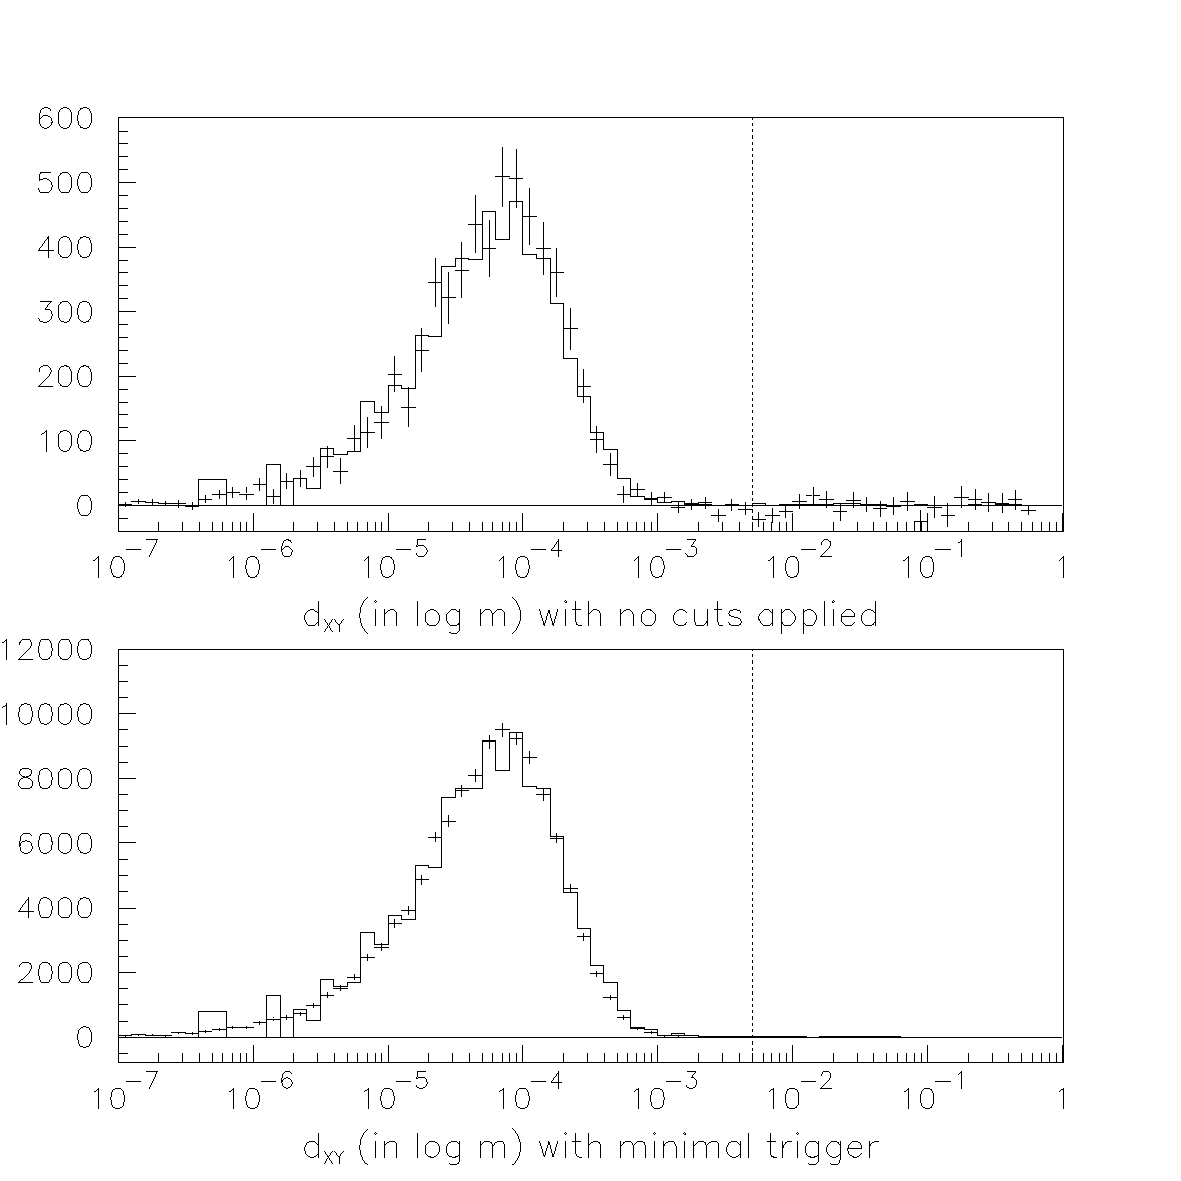
\includegraphics[width=\linewidth]{plots/cascades_logd0close}
  \caption{\label{cascades_logd0close} Closest track to beam spot XY
  in log $x$ scale ($\pi^+\pi^-$ removed, sideband-subtracted),
  without any cuts (top) and after requiring the minimal trigger
  (bottom).  The dotted line is the cut boundary, and the solid
  histogram is Monte Carlo.}
\end{figure}

\begin{figure}[p]
  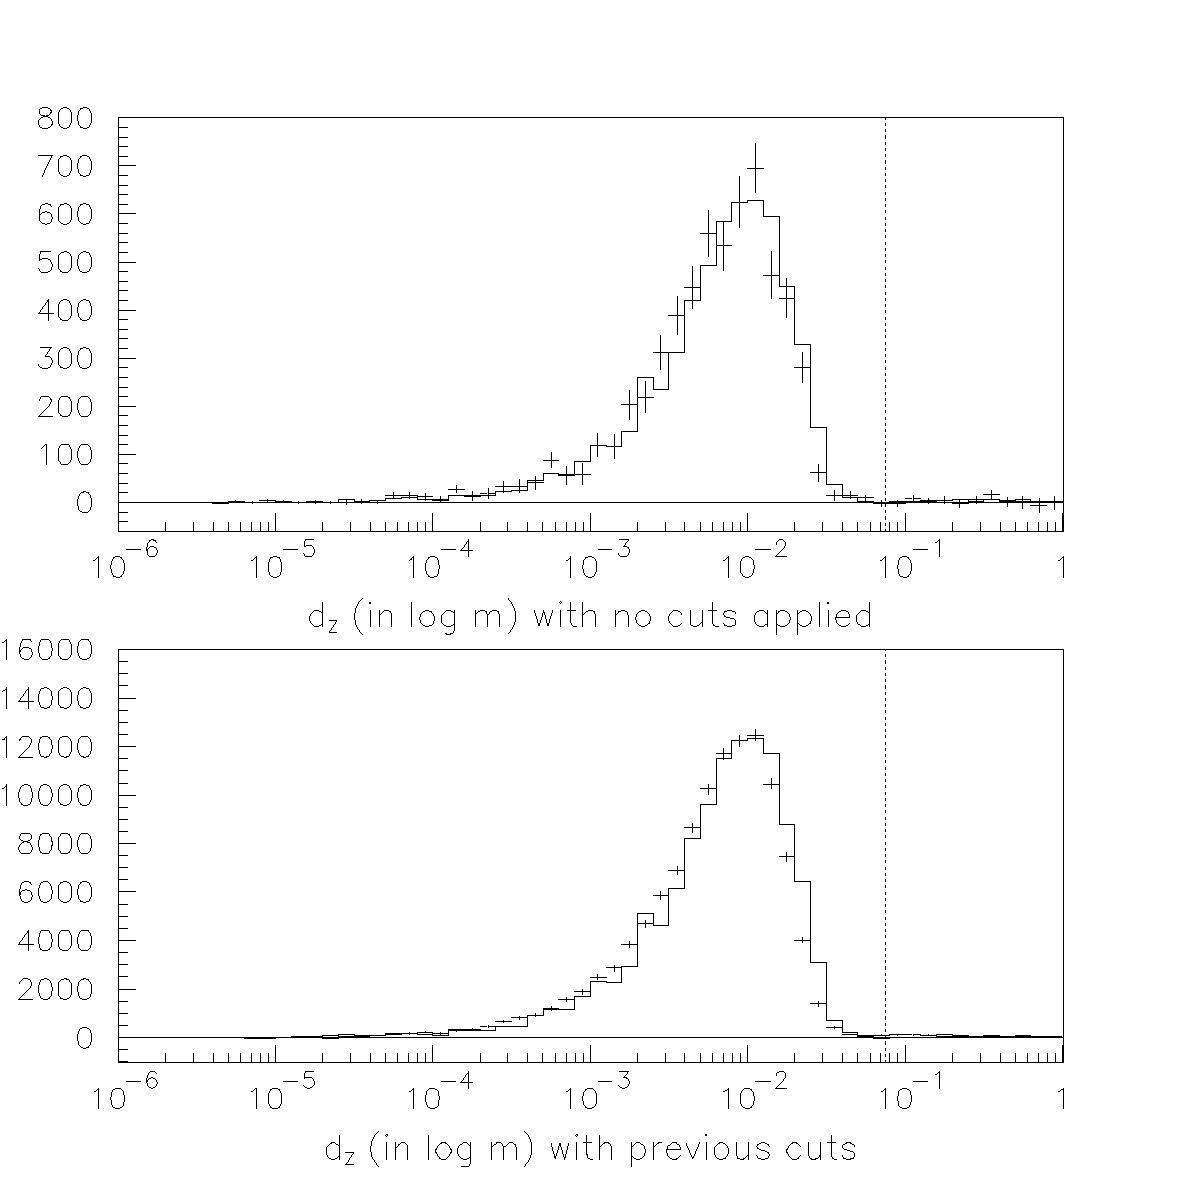
\includegraphics[width=\linewidth]{plots/cascades_logwz}
  \caption{\label{cascades_logwz} Z of primary vertex in log $x$ scale
  ($\pi^+\pi^-$ removed, sideband-subtracted), without any cuts (top)
  and after requiring previous cuts (bottom).  The dotted line is the
  cut boundary, and the solid histogram is Monte Carlo.}
\end{figure}

\begin{figure}[p]
  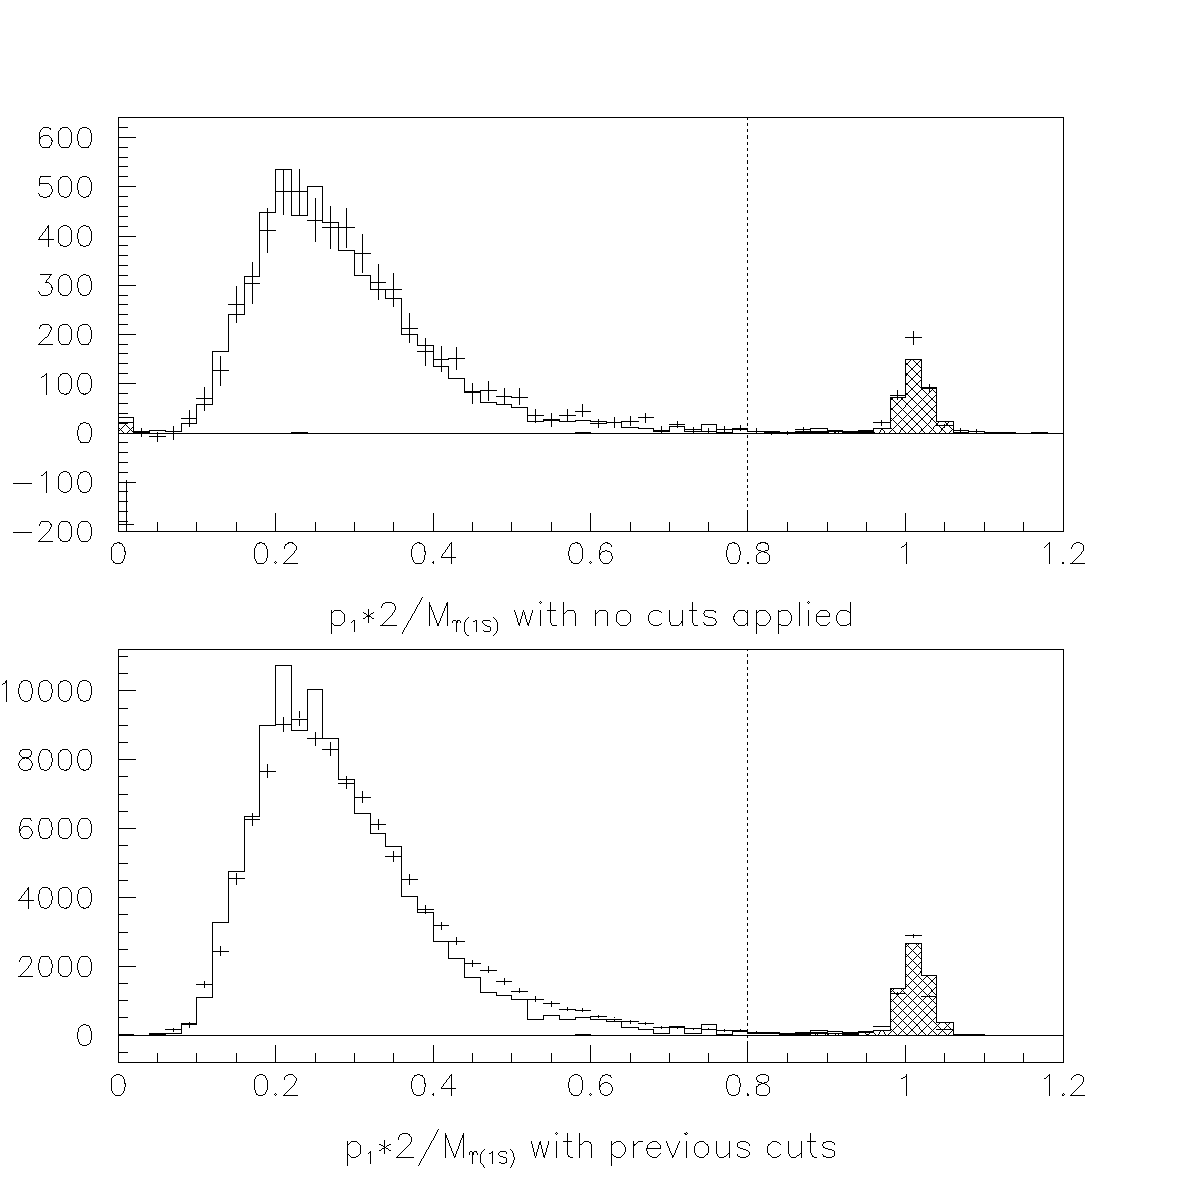
\includegraphics[width=\linewidth]{plots/cascades_p1}
  \caption{\label{cascades_p1} Momentum of biggest track divided by
  $M_{\Upsilon(1S)}/2$ ($\pi^+\pi^-$ removed, sideband-subtracted),
  without any cuts (top) and after requiring previous cuts (bottom).
  The dotted line is the cut boundary, and the solid histogram is
  Monte Carlo.  The cross-hatched histogram is Monte Carlo
  $\Upsilon(1S) \to e^+e^-$ and $\mu^+\mu^-$.}
\end{figure}

\begin{figure}[p]
  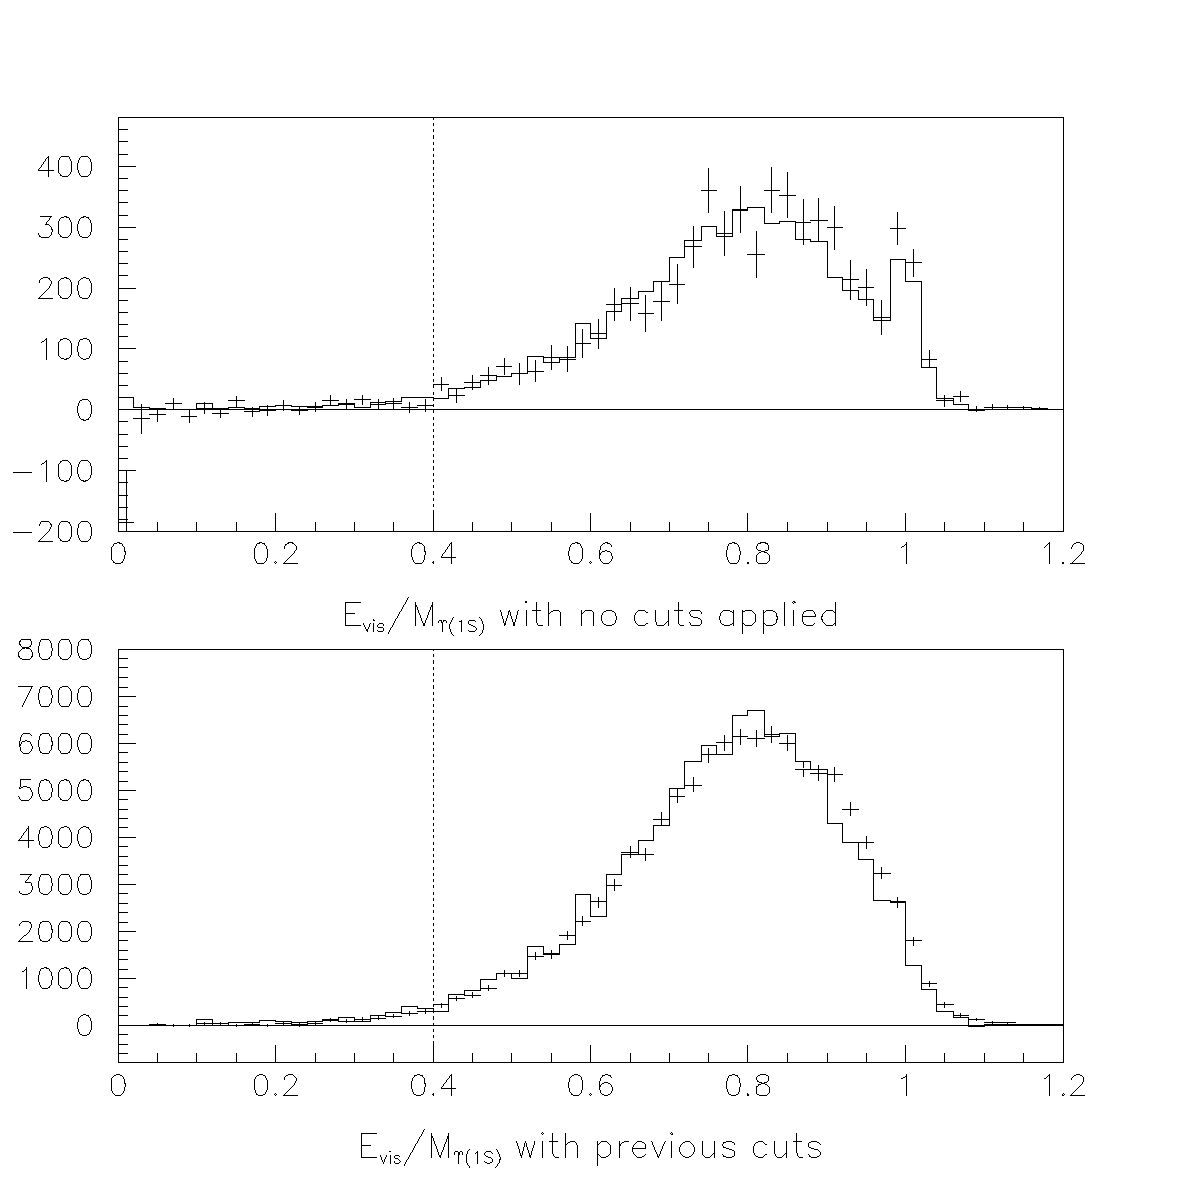
\includegraphics[width=\linewidth]{plots/cascades_visen}
  \caption{\label{cascades_visen} Visible energy divided by
  $M_{\Upsilon(1S)}$ ($\pi^+\pi^-$ removed, sideband-subtracted),
  without any cuts (top) and after requiring previous cuts (bottom).
  The dotted line is the cut boundary, and the solid histogram is
  Monte Carlo.}
\end{figure}

\begin{figure}[p]
  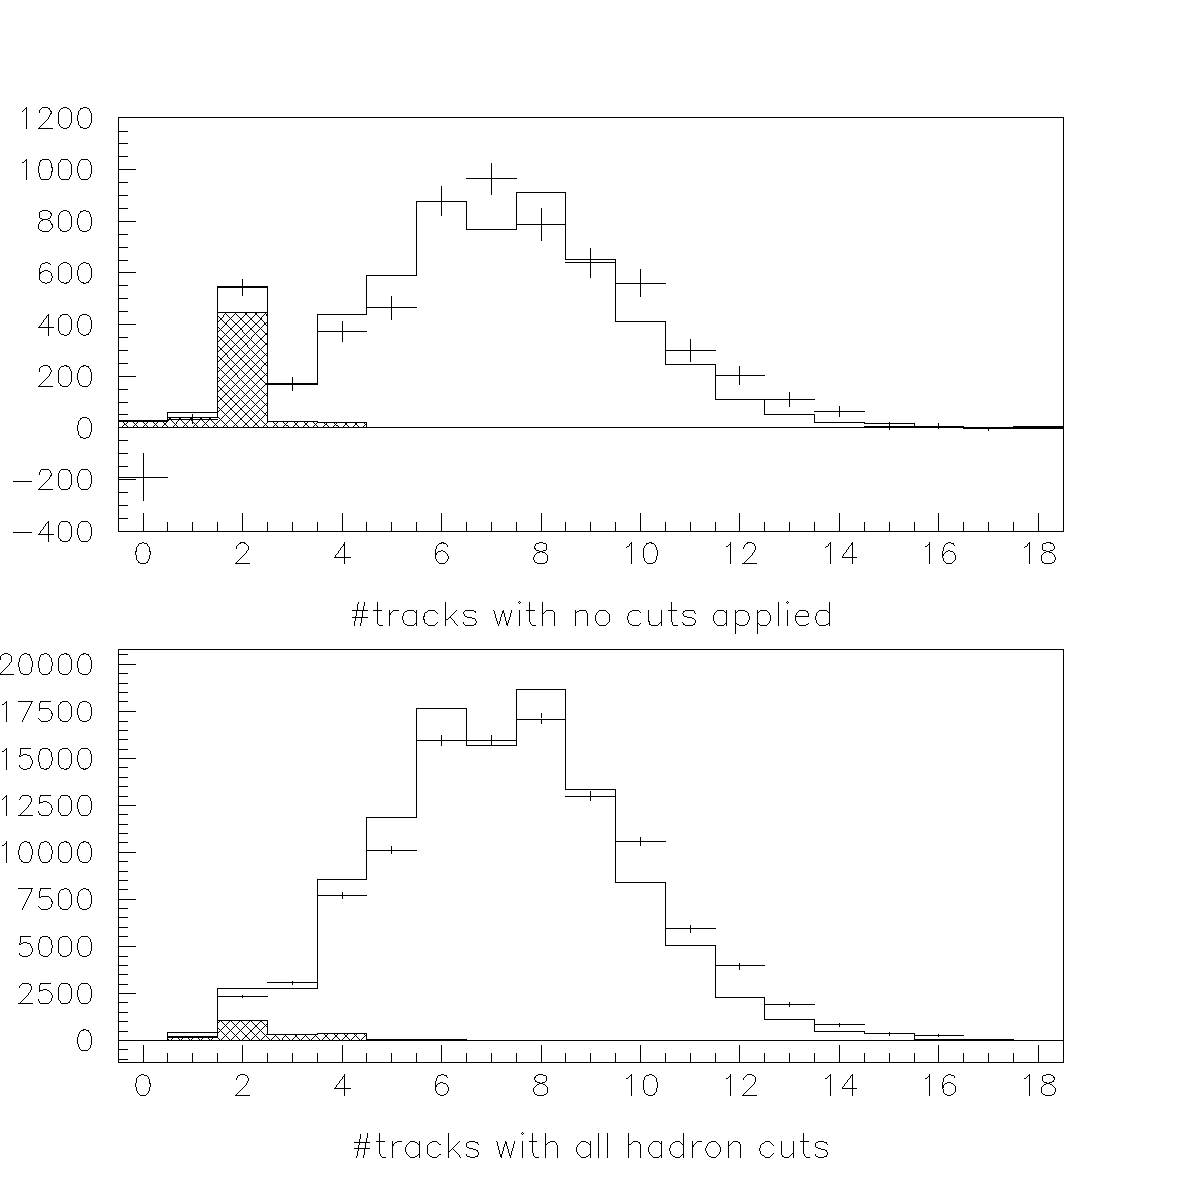
\includegraphics[width=\linewidth]{plots/cascades_tracks}
  \caption{\label{cascades_tracks} Number of quality tracks
  ($\pi^+\pi^-$ removed, sideband-subtracted), without any cuts (top)
  and after requiring all hadron cuts (bottom).  The solid histogram
  is Monte Carlo, and the cross-hatched histogram is Monte Carlo
  $\Upsilon(1S) \to e^+e^-$, $\mu^+\mu^-$, and $\tau^+\tau^-$ (in
  the bottom plot, almost entirely $\tau^+\tau^-$).}
\end{figure}

In Table \ref{cascades_table}, cut efficiencies have been calculated
by counting events with the cut applied ($A$), counting events with
the negation of the cut applied ($B$) and reporting
\begin{equation}
  \frac{A}{A+B} \pm \frac{\sqrt{{\sigma_A}^2 B^2 + {\sigma_B}^2
  A^2}}{(A+B)^2} \mbox{.}
\end{equation}
These statistical uncertainties have been added in quadrature with
sideband fit uncertainties (which were usually smaller than 0.05\%).
Cumulative cuts either have the minimal trigger applied or the maximal
trigger applied; the value I quote is the average of the two with half
the difference added in quadrature to the error.  (This correction is
also usually smaller than the statistical uncertainties.)

The minimal trigger efficiency in data is 102.5 $\pm$ 1.9\%; it has
statistically fluctuated above the maximum allowed value of 100\%.
(The sideband subtraction made this possible.)  The probability
distribution for the trigger efficiency is
\begin{equation}
  P(\varepsilon) = \exp(-(\varepsilon - 102.5)^2/2/1.9^2) / \sqrt{2 \pi} / 1.9 \mbox{,}
\end{equation}
so if I impose the constraint that the efficiency cannot be above
100\%, only the tail below 100\% remains (9.4\% of the a priori
probability).  This distribution has a mean and standard deviation of
99.11 $\pm$ 0.77\%.  This is what I will quote as the value and error
of the minimal trigger efficiency in data, though I'm sufficiently
uncomfortable about it that I devote the next Chapter to measuring the
trigger efficiency by other means.

The maximal trigger efficiency {\it given} the minimal trigger is very
well known in data (99.55 $\pm$ 0.12\%) because some of the background
is suppressed and this measurement comes from a data sample which is
not prescaled.  Therefore I compute the total efficiency of the
maximal trigger by applying
\begin{equation}
  P(\mbox{maximal trigger}) = P(\mbox{maximal trigger} | \mbox{minimal
  trigger}) \times P(\mbox{minimal trigger})\mbox{.}
\end{equation}
The Monte Carlo has much smaller backgrounds, so its maximal trigger
efficiency can be measured directly.

The most precise measurements of cut efficiency are cumulative, the
efficiency of each cut with all previous cuts applied.  These have
been listed between the two horizontal lines in Table
\ref{cascades_table}.  The total efficiency is just the product of
these times the trigger efficiency, though I can avoid
multiply-counting errors by measuring the efficiency of all cuts
except the trigger as a single cut.  This is presented below the
second line in the Table.  For the efficiency of all cuts, I must
multiply by the trigger efficiency, which is assumed to be the average
of the minimal and maximal trigger efficiencies with half the
difference as error.  (In data, the minimal and maximal trigger
efficiencies have almost entirely correlated errors, so this error is
counted only once.)

\begin{table}
  \caption{\label{cascades_table} Efficiency of each cut in cascade
  data, cascade Monte Carlo, and direct $e^+e^- \to \Upsilon(1S)$
  Monte Carlo.  Each line includes all decay modes except when
  otherwise noted.  Direct Monte Carlo errors are in the last digit
  presented.}
  \begin{center}
    \begin{tabular}{p{0.4\linewidth} c c c}
      & data & Monte Carlo & direct $\Upsilon$ \\\hline
      minimal trigger                	     & 99.11 $\pm$ 0.77\%   & 98.77 $\pm$ 0.17\% & \\
      maximal trigger                	     & 98.66 $\pm$ 0.78\%   & 97.77 $\pm$ 0.54\% & \\
      true trigger                   	     &                      &                    & 98.50\% \\\hline
      \dxy\ $<$ 5 mm given trigger   	     & 99.951 $\pm$ 0.031\% & 99.89 $\pm$ 0.13\% & 99.97\% \\
      \dz\ $<$ 7.5 cm given previous 	     & 99.23 $\pm$ 0.15\%   & 99.64 $\pm$ 0.21\% & 99.81\% \\
      \pone\ $<$ 80\% \ebeam\ given previous & 94.68 $\pm$ 0.21\%   & 93.48 $\pm$ 1.0\%  & 95.04\% \\
      \pone\ (hadronic decays)               & 99.72 $\pm$ 0.27\%   & 99.80 $\pm$ 0.21\% & 99.87\% \\
      \visen\ $>$ 40\% \ecom\ given previous & 98.90 $\pm$ 0.28\%   & 98.05 $\pm$ 0.62\% & 98.78\% \\\hline
      everything given trigger               & 92.87 $\pm$ 0.42\%   & 91.2 $\pm$ 1.3\%   & \\
      assumed trigger efficiency             & 98.89 $\pm$ 0.78\%   & 98.27 $\pm$ 0.56\% & \\
      everything                             & 91.84 $\pm$ 0.84\%   & 89.6 $\pm$ 1.3\%   & 93.89\% \\
      everything (hadronic decays)           & 97.68 $\pm$ 0.92\%   & 98.37 $\pm$ 0.61\% & 98.72\% \\
    \end{tabular}
  \end{center}
\end{table}

For two cuts (``\pone\ $<$ 80\% \ebeam'' and ``everything''), I want
to calculate the efficiency of only hadronic decay modes: all modes
except $\Upsilon(1S) \to e^+e^-$, $\mu^+\mu^-$, and $\tau^+\tau^-$.
For this I rely on previous measurements of the $\Upsilon(1S)$
branching fractions and the Monte Carlo's simulation of the leptonic
decays.  Without assuming lepton universality, these branching
fractions are
\begin{eqnarray}
  \mathcal{B}_{ee} &=& 2.38 \pm 0.11\% [\ref{cite:pdg}] \\
  \mathcal{B}_{\mu\mu} &=& 2.49 \pm 0.07\% [\ref{cite:istvan}] \\
  \mathcal{B}_{\tau\tau} &=& 2.67 \pm 0.15\% [\ref{cite:pdg}] \mbox{.}
\end{eqnarray}
From
\begin{equation}
  \varepsilon_\subs{all modes} = \varepsilon_\subs{had}
  (1 - \mathcal{B}_{ee} - \mathcal{B}_{\mu\mu} -
  \mathcal{B}_{\tau\tau}) + \varepsilon_{ee} \mathcal{B}_{ee} +
  \varepsilon_{\mu\mu} \mathcal{B}_{\mu\mu} + \varepsilon_{\tau\tau}
  \mathcal{B}_{\tau\tau}
\end{equation}
I can derive
\begin{equation}
  \varepsilon_\subs{had} = \frac{\varepsilon_\subs{all modes} -
  \varepsilon_{\tau\tau} \mathcal{B}_{\tau\tau}}{1 - \mathcal{B}_{ee}
  - \mathcal{B}_{\mu\mu} - \mathcal{B}_{\tau\tau}}
\end{equation}
by assuming that $\varepsilon_{ee}$ and $\varepsilon_{\mu\mu}$ are
zero.  (They are less than 0.3\% for the cuts in question.)  For the
\pone\ cut alone, $\varepsilon_{\tau\tau}$ is 93\%, and for
everything, $\varepsilon_{\tau\tau}$ is 57\%.  In these two cases, the
propagated error is
\begin{equation}
  \sqrt{2.41\times 10^{-6} + (-5.56 + 5.40 {\varepsilon_\subs{all modes}})\times 10^{-6} {\varepsilon_\subs{all modes}} + 1.17 {\sigma_{\varepsilon_\subs{all modes}}}^2}
\end{equation}
and
\begin{equation}
  \sqrt{0.91\times 10^{-6} + (-3.41 + 5.40 {\varepsilon_\subs{all modes}})\times 10^{-6} {\varepsilon_\subs{all modes}} + 1.17 {\sigma_{\varepsilon_\subs{all modes}}}^2} \mbox{,}
\end{equation}
respectively.  In Monte Carlo, I simply turn off leptonic decays, and
gain significantly in precision.

\section{Cascade Contributions to Efficiency Measurement}

From the Table, I conclude that the most problematic translations from
cascade efficiencies to direct $e^+e^- \to \Upsilon(1S)$ efficiencies
are due to the leptonic modes.  With these removed, cascade data and
cascade Monte Carlo agree on every cut efficiency, as do cascade Monte
Carlo and direct Monte Carlo.  But this may only be because the
cascade data and cascade Monte Carlo are couched in large
uncertainties.

The cascades study puts limits on errors introduced by using the Monte
Carlo for cut efficiencies.  The uncertainties presented in Table
\ref{cascades_contributions} are derived from adding the cascade
data--cascade Monte Carlo differences in quadrature with their errors.

\begin{table}[!ht]
  \caption{\label{cascades_contributions} Uncertainties in Monte Carlo
  modeling of hadronic decays for each cut}
  \begin{center}
    \begin{tabular}{p{0.5\linewidth} c}
      trigger                                   & 1.34\% \\
      \dxy\ $<$ 5 mm   	   		        & 0.15\% \\
      \dz\ $<$ 7.5 cm 	   		        & 0.48\% \\
      \pone\ $<$ 80\% \ebeam\ (hadronic decays) & 0.35\% \\
      \visen\ $>$ 40\% \ecom                    & 1.09\% \\
      \lfourdec                                 & not measured with cascades \\
    \end{tabular}
  \end{center}
\end{table}

The trigger efficiency can be more tightly bound using a different set
of arguments, to be presented in the next chapter.  The trigger
efficiency in this study deviates from 100\% primarily because of the
leptonic final states, which can fail to trigger when they miss the CC
barrel.  Removing the lepton modes can improve the Monte Carlo
cascades measurement, but not the data cascades measurement.

The second-to-last cut, ``\visen\ $>$ 40\% \ecom,'' will be handled
differently because the cascade Monte Carlo uncertainties are too
large for a good comparison.  It will be measured using both the
unfiltered dataset and this cascades study.  The unfiltered dataset
has a large background of two-photon events at visible energies below
30\% \ecom, so I will only use the unfiltered dataset to measure the
30--40\% part.  The cascades dataset tells me that 0.28\% $\pm$ 0.19\%
of $\Upsilon(1S)$ events have visible energy below 30\%.  I will
simply add the two measurements to find out how many $\Upsilon$ decays
generate 0--40\% \visen/\ecom.

The last cut, \lfourdec, is too complicated to consider removing the
two pions, so it is left entirely to the unfiltered dataset.
